\documentclass{article}

\usepackage[hidelinks]{hyperref}
\urlstyle{same}

\usepackage{fontspec}

\setmonofont[
  Path=fonts/,
  BoldFont=MonaspaceKrypton-Bold.otf,
  ItalicFont=MonaspaceKrypton-Italic.otf,
  BoldItalicFont=MonaspaceKrypton-BoldItalic.otf
]{MonaspaceKrypton-Regular.otf}

\usepackage{amsmath, amssymb}

\usepackage{graphicx}
\graphicspath{{images/}}

\usepackage[
  top=1cm,
  left=1cm,
  right=1cm,
  bottom=2cm,
  footskip=0.7cm
]{geometry}

\usepackage{listings}
\usepackage{xcolor}

\definecolor{lstbg}{RGB}{248,248,248}
\definecolor{lstframe}{RGB}{220,220,220}
\definecolor{lstkeyword}{RGB}{0,92,197}
\definecolor{lstcomment}{RGB}{0,128,0}
\definecolor{lststring}{RGB}{163,21,21}
\definecolor{lstnumber}{RGB}{120,120,120}

\lstdefinestyle{cppstyle}{
  language=cpp,
  backgroundcolor=\color{lstbg},
  frame=single,
  rulecolor=\color{lstframe},
  frameround=tttt,
  basicstyle=\ttfamily\small,
  keywordstyle=\color{lstkeyword}\bfseries,
  commentstyle=\color{lstcomment}\itshape,
  stringstyle=\color{lststring},
  numberstyle=\tiny\color{lstnumber},
  numbers=left,
  stepnumber=1,
  numbersep=8pt,
  showstringspaces=false,
  breaklines=true,
  breakatwhitespace=true,
  columns=fullflexible,
  keepspaces=true,
  tabsize=4,
  upquote=true
}

\lstdefinelanguage{cpp}{
  language=[11]C++,
  morekeywords={concept,consteval,constinit,co_await,co_return,co_yield,requires},
  sensitive=true
}

\lstset{style=cppstyle}

\title{C++ Cheatsheet}
\author{Daniel Sinkin}
\date{\today}

\begin{document}

\maketitle

\tableofcontents
\newpage

\section{Introduction}
This document contains my notes on C++ specifics I'm reviewing for my job application.

\section{Changes per version}
\subsection{C++26}
\subsubsection{Contracts}
Will introduce Contracts which give an explicit syntax to implement post and pre conditions
(formalising \texttt{gsl::Expects} and \texttt{gsl::Ensures}) as well as a new more stable assert syntax in
form of \texttt{contract\_assert}.

\begin{lstlisting}[language=cpp,caption={Pre-C++26: gsl::Expects/gsl::Ensures + assert}]
auto div_round_down_pos(std::int32_t a, std::int32_t b) -> std::int32_t
{
    gsl::Expects(a > 0);
    gsl::Expects(b > 0);

    const std::int32_t r = a / b;
    assert((r + 1) * b > a);

    Ensures(r * b <= a);
    return r;
}
\end{lstlisting}

\begin{lstlisting}[language=cpp,caption={C++26: Contract syntax}]
auto div_round_down_pos(std::int32_t a, std::int32_t b) -> std::int32_t 
    pre  (a > 0)
    pre  (b > 0)
    post (r * b <= a)
{
    contract_assert((r + 1) * b > a);
    const std::int32_t r = a / b;
    return r;
}
\end{lstlisting}

\subsubsection{Anonymous values}
Sometimes we don't care about the name of a variable but still have to assign it, in the past you'd need to make up a (unique) name for the variable, now you can just use \texttt{\_}.

\begin{lstlisting}[language=cpp,caption={C++26: Anonymous values}]
auto& [_, value] = f(); // Structured binding

Mutex m1{}, m2{};
{
    std::scoped_lock _{m1, m2}; // RAII utils
}
\end{lstlisting}

\subsection{C++23}
\subsubsection{std::expected}
Allows for functional / Rust style errors as values.

\begin{lstlisting}[language=cpp,caption={C++26: Anonymous values}]
enum class MyError {
    negative_number;
    zero_division;
}

std::expected<float, PositiveDivisionError> my_div(float a, float b) {
    if((a * b) <= 0.0f) {
        return std::unexpected{MyError:negative_number};
    }
    if(b == 0.0f) {
        return std::unexpected{MyError:zero_division};
    }
    return a / b;
}

int main() {
    auto res = my_div(5.0, 3.0);
    if(!res) {
        switch(res.err()) {
            case MyError::negative_number: {/*...*/}
            case MyError::zero_division: {/*...*/}
        }
    } else {
        float value{*res};
        /* ... */
    }
}

\end{lstlisting}

\subsubsection{std::print, std::println}
Introduced \texttt{print} which allows for structured printing by leveraging the C++20 feature \texttt{std::format}.

\begin{lstlisting}[language=cpp,caption={std::println}]
std::println("Hello, {}. The value of x is {}", "World", 5);
\end{lstlisting}

\subsubsection{std::generator}
\url{https://www.youtube.com/watch?v=7ZazVQB-RKc}

Can access like normal iterators
\subsection{C++20}
\subsubsection{std::format}
Introduced \texttt{std::format} which allows for formatting of variables into strings.

\begin{lstlisting}[language=cpp,caption={std::format}]
float x = 12.52343232f;
std::string s{std::format("x = {:.2f}", x)}; // s == "x = 12.52"
\end{lstlisting}

\subsubsection{Concepts}
Compile time constraints on templates, reducing the need for SFINAE boilerplate
\begin{lstlisting}[language=cpp,caption={std::format}]
template <std::integral T>
T add(T a, T b) { return a + b; }
\end{lstlisting}

\subsubsection{Ranges}
\subsubsection{Coroutines}
\begin{lstlisting}
co_await task;
co_yield value;
\end{lstlisting}

\subsubsection{Modules}
Adoption of those is horrible so far.

\subsubsection{Calendar support for std::chrono}
\begin{lstlisting}[language=cpp,caption={Pre-C++17: std::array without CTAD}]
using namespace std::chrono;
auto zt = zoned_time{"Europe/Berlin", system_clock::now()};
\end{lstlisting}

\subsection{C++17}
\subsubsection{CTAD (Class Template Argument Deduction)}
Made template type deduction possible for class templates.
\begin{lstlisting}[language=cpp,caption={Pre-C++17: std::array without CTAD}]
#include <array>

std::array<int, 3> values{{1, 2, 3}};
\end{lstlisting}

\begin{lstlisting}[language=cpp,caption={C++17: std::array with CTAD}]
#include <array>

std::array values{1, 2, 3}; // std::array<int, 3>
\end{lstlisting}

\subsubsection{std::scoped\_lock}
An improvement on \texttt{std::lock\_guard} which allows to lock multiple mutexes in one call.

\begin{lstlisting}[language=cpp,caption={std::scoped\_lock}]
std::mutex m1, m2;
{
    std::scoped_lock locks{m1, m2};
}
\end{lstlisting}

\subsection{C++14}
\subsubsection{constexpr loops and conditionals}
Added support for loops and if/else branches.
\begin{lstlisting}[language=cpp,caption={C++14: constexpr with loops and conditionals}]
constexpr int sum_up_to(int n)
{
    int result = 0;

    for (int i = 1; i <= n; ++i)   // constexpr loop (C++14)
    {
        if (i % 2 == 0)            // constexpr conditional (C++14)
        {
            result += i;
        }
    }

    return result;
}
\end{lstlisting}
\subsection{C++11}
\subsubsection{Value Semantics}
Added move semantics and rvalue references.
\begin{lstlisting}[language=cpp,caption={Move constructors, Move assignment}]
std::vector<int> a = make_vector();
\end{lstlisting}

\begin{lstlisting}[language=cpp,caption={RAII}]
struct File {
    File(const char* path);
    ~File();
    File(File&&);
    File& operator=(File&&);
};
\end{lstlisting}

\subsubsection{constexpr}
Allows for compile time execution of code, for example offloading computations to compile time. Support was very sparse at this point and got continually extended.

\begin{lstlisting}[language=cpp,caption={constexpr (initial form)}]
constexpr float k_pi = 3.14f;

constexpr int square(int x) {
    return x * x;
}
\end{lstlisting}

\subsubsection{Lambdas}
\begin{lstlisting}[language=cpp,caption={C++11 Lambda}]
auto f = [](int x) {
    return x * x;
};
\end{lstlisting}

\subsubsection{std::unordered\_map}

\subsubsection{std::lock\_guard}
\begin{lstlisting}[language=cpp,caption={Lock Guard}]
Mutex x;
{
    std::lock_guard<Mutex> guard{x};
}
\end{lstlisting}

\newpage
\section{C++ Concepts}
\subsection{Value Semantics}
Every Expression belongs to one of the following value categories:
\begin{itemize}
\item L value
\item PR Value (Pure R value)
\item X Value (eXpiring value)
\end{itemize}
When it is an L value or a X value we call it a GL (General L) value, if it is a PR value or a X value we call it a R value. In particular X values are both GL and R values. The naming is a bit unfortunate, it should PL value and L value; or GR value and R value.

Names are inspired by the fact that L values sit on the "left side of assignments" and R values sit on the "right side of assignments" and are temporaries in that sense. More concretely a L value is something that has a set memory location (\texttt{\&x} or more accurately \texttt{std::address\_of(x)}) which can be accessed. An R value is a temporary that does not have an addressable memory location (due to temporary materialisation this is no longer true, but an analogy to think about). X values are GL values which represent expiring objects, so they currently have a fixed memory handle but that one has a "soon" ending lifetime.
\begin{lstlisting}[language=cpp,caption={Rule of 5}]
int x = 5;
x; // This id-expression is an L value
(x); // L value
&x; // prvalue of type int*

1 + 1; // prvalue (of type int)

struct Foo {/*...*/}
Foo foo{}; // declaration not an expression, so no value cateogry

foo; // lvalue
f(foo); // passes an L value 
f(std::move(foo)); // X value
f(Foo{}); // passes an PR value 
\end{lstlisting}

\subsubsection{Perfect Forwarding}
Under the hood \texttt{std::forward} is implemented as a cast:
\begin{lstlisting}
template <class T>
constexpr T&& forward(std::remove_reference_t<T>& t) noexcept
{
    return static_cast<T&&>(t);
}

template <class T>
constexpr T&& forward(std::remove_reference_t<T>&& t) noexcept
{
    static_assert(!std::is_lvalue_reference_v<T>,
                  "bad forward: cannot forward an rvalue as an lvalue");
    return static_cast<T&&>(t);
}
\end{lstlisting}

\begin{lstlisting}
class Foo{ /*...*/ };

void kind(T) { println("1"); }
void kind(const T&) { println("2"); }
void kind(T&&) { println("3"); }

template <typename T>
void bad_forward(T &&arg)
{
    kind(arg);
}

template <typename T>
void good_forward(T &&arg)
{
    kind(std::forward<T>(arg));
}

int main()
{
    Foo f{};
    bad_forward(f);        // prints: kind(Foo&)
    bad_forward(Foo{});    // prints: kind(Foo&)
    good_forward(f);       // prints: kind(Foo&)
    good_forward(Foo{});   // prints: kind(Foo&&)
}
\end{lstlisting}

\subsection{Resource Ownership}
\subsubsection{Rule of Five}
If you implement any of the following then you should implement all of them. The reasoning behind that is that you implementing a non-standard constructor or destructor implies that you have some non-trivial resource you don't trust the compiler to manage properly (e.g. heap allocations, database connection, file handle). This used to be the Rule of Three but now we have move and copy assignment constructors since C++11.
\begin{lstlisting}[language=cpp,caption={Rule of 5}]
class Foo {
    Foo() {}
    ~Foo() {...} // Destructor
    Foo(const Foo&) {...} // Copy Constructor
    Foo(Foo&&) {...} // Move Constructor
    Foo& operator=(const Foo&) {...} // Copy assignment constructor
    Foo& operator=(Foo&&) {...} // Move assignment constructor
}
\end{lstlisting}

\subsubsection{Rule of Zero}
Given that implementingi the Rule of Five is annoying and creates a lot of boilerplate one should avoid that whenever possible, that is the Rule of Zero.

\subsubsection{RAII (Resource Acquisition is Initialisation)}
In my opinion this is a terrible name and should instead be CADR (Constructor Acquires Destructor Releases). It is a type of scope based automatic resource cleanup, the main idea is that when you invoke the constructor you obtain some resource which you hold for the entire lifetime of that class and once that lifetime has passed (on leaving scope) the resource gets automatically released. This is for example how one can use \texttt{std::vector} to avoid having to manually call \texttt{new} and \texttt{delete}.

To employ this we define a class with a constructor which allocates memory on the heap and a destructor which frees this memory.
\begin{lstlisting}
class RAII {
    RAII(std::string_view name) : name_(name), data_(static_cast<int*>(std::malloc(8 * sizeof(int)))) {
        std::println("Allocated Memory '{}'", name_);
    }
    ~RAII() {
        std::free(data_);
        std::println("Deallocated Memory '{}'", name_);
    }
private:
    std::string name_{};
    int* data_{};
};
\end{lstlisting}
we then can't leak memory anymore, even if exceptions get thrown:
\begin{lstlisting}
auto func() -> void {
    std::println("Starting Function");
    RAII func_scope("Function Scope");
    std::println("Starting inner scope");
    {
        RAII inner_scope("Inner Scope");
    }
    std::println("Finished inner scope");
    std::println("Throwing exception");
    throw std::runtime_error("");

    std::println("Finished function");
}

int main() {
    std::println("Starting Program");
    try {
        func();
    } catch (...) {
        std::println("Caught exception");
    }
    std::println("Finishing Program");
}
/*
Starting Function
Allocated Memory 'Function Scope'
Starting inner scope
Allocated Memory 'Inner Scope'
Deallocated Memory 'Inner Scope'
Finished inner scope
Throwing exception
Deallocated Memory 'Function Scope'
Caught exception
Finishing Program
*/
\end{lstlisting}

\texttt{scoped\_lock} and (the now outdated \texttt{lock\_guard}) are examples of RAII wrappers for mutexes, \texttt{std::vector} is a RAII wrapper around dynamic memory.

\subsection{NRVO (Named Return Value Optimisation)}
To show that NRVO happens we construct a simple tracker class which prints out whenever a copy / move / normal construction happens.
\begin{lstlisting}
using Data = std::array<int, 32>;
class TrackMemory {
public:
    TrackMemory() {
        std::println("Empty Constructor");
    }
    TrackMemory(const TrackMemory &other) : data_(other.data_) {
        std::println("Copy constructor");
    }
    TrackMemory(TrackMemory &&other) noexcept : data_(std::move(other.data_)) {
        std::println("Move constructor");
    }
private:
    Data data_{};
};
\end{lstlisting}
Now we want to show three different cases, one where NRVo can't happen (different named variables of the same type get returned)
\begin{lstlisting}
auto no_nrvo(bool return_a) -> TrackMemory {
    TrackMemory a{}, b{};
    if (return_a) { return a; }
    return b;
}
\end{lstlisting}
one where we, according to the standard, might have NRVO (returning a single named variable)
\begin{lstlisting}
auto possible_nrvo() -> TrackMemory {
    TrackMemory a{};
    return a;
}
\end{lstlisting}
and one case where we are forced to have RVO (case where we return an unnamed temporary)
\begin{lstlisting}
auto forced_nrvo() -> TrackMemory {
    return TrackMemory{};
}
\end{lstlisting}
We then run those
\begin{lstlisting}
int main() {
    std::println("Impossible NRVO:");
    auto tm = no_nrvo(0);
    // Empty Constructor
    // Empty Constructor
    // Move constructor
    std::println("\nPossible NRVO:");
    auto tm2 = possible_nrvo();
    // Empty Constructor
    std::println("\nForced NRVO:");
    auto tm3 = forced_nrvo();
    // Empty Constructor
}
\end{lstlisting}

\subsection{EBO (Empty Base Optimisation)}
\begin{lstlisting}
struct alignas(16) EmptyAligned {};

class NoEBO {
private:
    double data_{};
    EmptyAligned empty_interals_{};
};

class WithEBO {
private:
    double data_{};
    [[no_unique_address]] EmptyAligned empty_internals_{};
};

static_assert(std::is_empty_v<EmptyAligned>);
static_assert(sizeof(EmptyAligned) == 16);
static_assert(alignof(EmptyAligned) == 16);
static_assert(sizeof(NoEBO) == 32);
static_assert(sizeof(WithEBO) == 16);
\end{lstlisting}

\subsection{Idioms and Patterns}
\subsubsection{Two-pointer merge}
\url{https://en.wikipedia.org/wiki/Merge_algorithm}

If you want to merge two streams or lists together with some inequality relation on the values you do this:
\begin{lstlisting}
std::vector<int> a{/*...*/};
std::vector<int> b{/*...*/};
std::vector<int> c{};
c.reserve(a.size() + b.size());

auto it_a = a.begin();
auto it_b = b.begin()
while(it_a != a.end() && it_b != b.end()) {
    if(*it_a <= *it_b) {
        c.push_back(*it_a);
        ++it_a;
    } else {
        c.push_back(*it_b);
        ++it_b;
    }
}
while(it_a != a.end()) {
    c.push_back(*it_a);
    ++it_a;
}
while(it_b != b.end()) {
    c.push_back(*it_b);
    ++it_b;
}
\end{lstlisting}

\subsubsection{Lazy Delete Idiom / Tombstoning}
When you want to delete an object in the middle (or beginning) of a vector you first have to push that element to the end and shift everything to the left by 1 and then \texttt{pop\_back}, this can be very expensive, especially if many objects have to be deleted.

A common trick to avoid this is to keep a list of tombstones which are boolean values denoting if that value is deleted, and when you access or iterate you simply skip those elements.

If you occassionally pop elements off the back it can be advantageous to just keep popping as long as there are tombstone objects on the top, or if you have downtime in your program you could do cleanup (batching the removal is much faster) or just keep the tombstoned values if the memory cost is not too high.
\begin{lstlisting}
struct DeleteableInt{
    int value{};
    bool is_deleted{false};
};

std::vector<DeletableInt> vec{};
vec.resize(100);
for(auto i = 0; i < vec.size(); ++i) {
    if(i & 1 == 0) {
        vec[i].is_deleted = true;
    }
}
\end{lstlisting}

\subsubsection{Scope Guard / Defer Pattern}
RAII wrappers can also be useful when trying to do some post-scope cleanup or operation, as a type of soft `texttt{defer}`.  For example I use 
\begin{lstlisting}
using Clock = std::chrono::steady_clock;
using TimePoint = Clock::time_point;
using Duration = std::chrono::duration<f64>;

ScopeTimer::ScopeTimer(std::string_view label) noexcept : label_(label), start_(Clock::now()) {}
ScopeTimer::~ScopeTimer() noexcept
{
    const auto dt = Clock::now() - start_;
    const auto seconds = std::chrono::duration<f64>(dt).count();
    std::println("{}: {:.3f} ms", label_, seconds * 1000.0);
}
\end{lstlisting}
to quickly time scopes (for example actual scoped or function invocations).

\subsubsection{Unsigned reverse iteration idiom (\texttt{i-- > 0})}
When iterating backwards with an unsigned index (e.g. \texttt{std::size\_t}),
\texttt{i >= 0} is always true, and \texttt{i--} can underflow.
The idiom
\[
\texttt{for (auto i = n; i-- > 0;)}
\]
means: compare the current value to 0, then decrement, but the loop body sees
the decremented value, running for indices \texttt{n-1, ..., 0}.

\begin{lstlisting}[language=cpp,caption={Reverse loop for unsigned indices (safe)}]
for (std::size_t i = v.size(); i-- > 0; )
{
    use(v[i]);
}
\end{lstlisting}

The range (C++20) based alternative to this is to use
\begin{lstlisting}
\texttt{for (auto\& x : std::views::reverse(v)) {...}}
\end{lstlisting}


\subsection{ODR (One Definition Rule)}
Use the \texttt{extern} keyword if you want to decalre a variable but not define it to avoid ODR. Since C++17 you can (and should) use inline for variables instead.

A very subtle ODR bug can occur when you compile some files with debug symbols set and some without.

\subsection{SIOF (Static Initialisation Order Fiasco)}
When you have two non-local objects (e.g. globals or function-local statics) which have dynamic initialisation (run code in their constructors) which live in different translation units (.cpp files) then the initialisation order between them is not specificied (standard only guarantees it within one translation unit (top-to-bottom)).
\begin{lstlisting}[caption={a.cpp}]
extern std::string g_name;

std::string make_greeting() { return "Hello " + g_name; }

std::string g_greeting = make_greeting();
\end{lstlisting}

\begin{lstlisting}[caption={b.cpp}]
std::string g_name = "Daniel";
\end{lstlisting}

Because \texttt{g\_greeting} depends on \texttt{g\_name} it might not have been initialised when you define it, so you'd run into UB. Note that if \texttt{a.cpp} would start with \texttt{std::string g\_name = "Steve"} it would be an ODR (one definition rule) violation not SIOF.

\subsection{Important STL algorithms}
\subsection{Templates}
\subsubsection{Variadic Templates}
\subsubsection{Template Metaprogramming}

\newpage
\section{STL (Standard Templating Library)}
\subsection{Iterators}
\subsubsection{Iterator Categories}

\begin{figure}[h!]
    \centering

    \newcommand{\iterheight}{3.5cm}

    \begin{minipage}{0.32\textwidth}
        \centering
        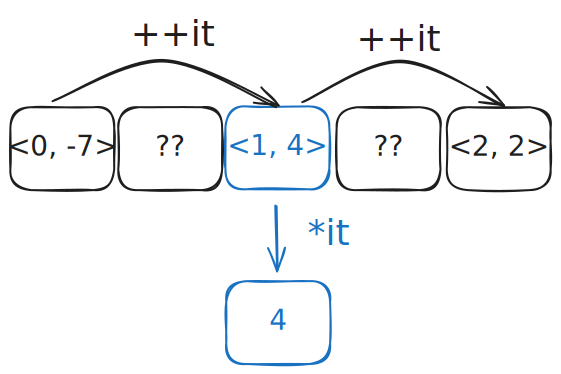
\includegraphics[height=\iterheight,keepaspectratio]{input_iterator.png}\\[0.3em]
        {\small Input iterator}
    \end{minipage}
    \hfill
    \begin{minipage}{0.32\textwidth}
        \centering
        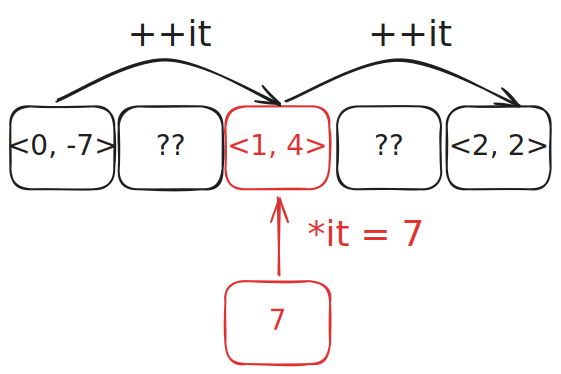
\includegraphics[height=\iterheight,keepaspectratio]{output_iterator.png}\\[0.3em]
        {\small Output iterator}
    \end{minipage}
    \hfill
    \begin{minipage}{0.32\textwidth}
        \centering
        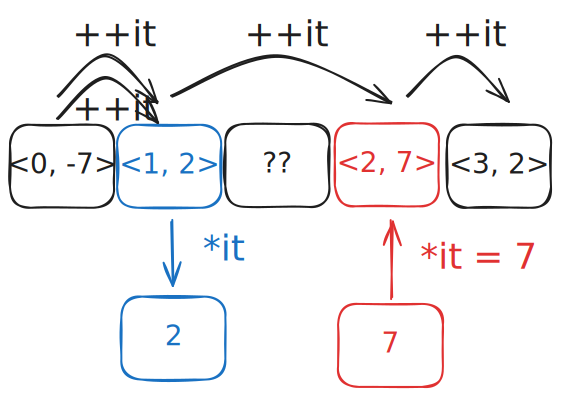
\includegraphics[height=\iterheight,keepaspectratio]{forward_iterator.png}\\[0.3em]
        {\small Forward iterator}
    \end{minipage}

    \caption{Single-pass and forward iterators}
\end{figure}

\begin{figure}[h!]
    \centering

    \newcommand{\iterheight}{3.5cm}

    \begin{minipage}{0.32\textwidth}
        \centering
        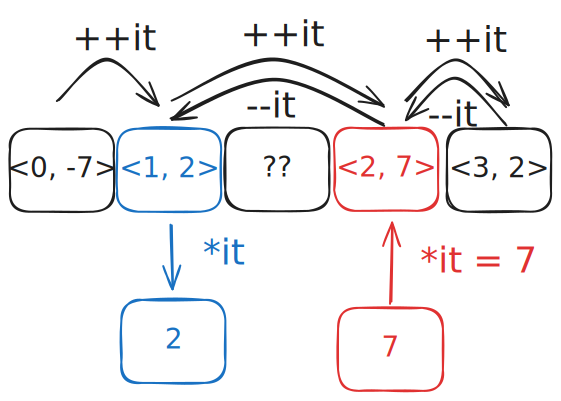
\includegraphics[height=\iterheight,keepaspectratio]{bidirectional_iterator.png}\\[0.3em]
        {\small Bidirectional iterator}
    \end{minipage}
    \hfill
    \begin{minipage}{0.32\textwidth}
        \centering
        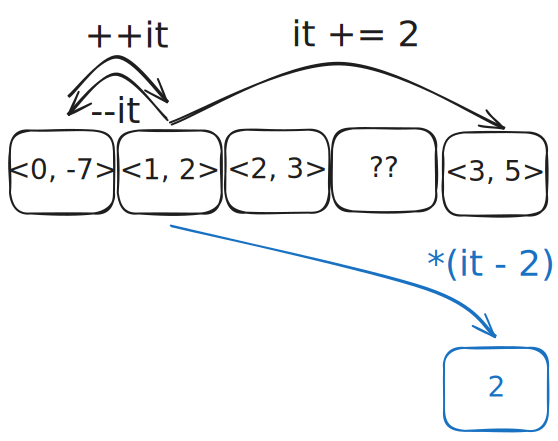
\includegraphics[height=\iterheight,keepaspectratio]{random_access_iterator.png}\\[0.3em]
        {\small Random-access iterator}
    \end{minipage}
    \hfill
    \begin{minipage}{0.32\textwidth}
        \centering
        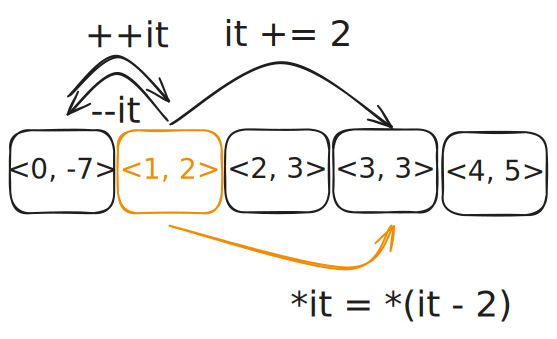
\includegraphics[height=\iterheight,keepaspectratio]{contiguous_iterator.png}\\[0.3em]
        {\small Contiguous iterator}
    \end{minipage}

    \caption{Bidirectional and stronger iterator categories}
\end{figure}

\subsection{Ranges}
First introduced in C++20, base don Eric Niebler's \texttt{Range-v3} library.
\subsubsection{Core Concepts}
\subsubsection{Views}
\texttt{std::ranges::filter}, \texttt{std::ranges::take}, \texttt{std::ranges::reverse}

For example the Unsigned reverse iteration idiom (\texttt{i-- > 0}) can be implemented using ranges instead:

\begin{lstlisting}
\texttt{for (auto\& x : std::views::reverse(v)) \{...\}}
\end{lstlisting}

\subsubsection{Range Algorithms}
\texttt{std::ranges::sort}, \texttt{std::ranges::find}, \texttt{std::ranges::copy}
\subsubsection{Range Concepts}

\subsection{Containers}
\subsection{Algorithms}

\newpage
\section{Data Structure implementations}
\subsection{std::vector (Trivially Copyable Types)}
A \texttt{vector<T>} is a heap allocated sequence container with three pointers \texttt{start\_}, \texttt{end\_}, \texttt{capacity\_}. The first denotes the start of the vector, the second the location AFTER(!) the last allocated elements and the third is the total memory we have allocated. They take up 24 bytes (\texttt{3 * sizeof(T*)}) of stack memory and \texttt{(capacity\_ - start\_) * sizeof(T)} bytes of heap memory.

The core operation on a vector is \texttt{push\_back} which takes an object and either inserts it in the back if there is space (\texttt{end\_} != \texttt{capacity\_}) or first resizes (doubling capacity on GCC and Clang, increasing it by 1.5 on MSVC) and then inserting in the end.

If you want to delete an element you swap that position with \texttt{end\_} and reduce \texttt{end\_} by one.

This is a famously badly named datastructure as it squats on the name of mathematicl elements of vector spaces and physics vectors. A better name would for example be DynamicArray.

\begin{lstlisting}[language=cpp,caption={Vector class}]
template <typename T>
class VectorTrivial
{
    static_assert(std::is_trivially_copyable_v<T>);
    
public:
    using size_type = std::size_t;
    /*Rule of 5*/
    /*Public API*/
private:
    T* start_{};
    T* end_{};
    T* cap_{};
    /*Private API*/
};
\end{lstlisting}

\subsubsection{Rule of 5}
\begin{lstlisting}[language=cpp,caption={Rule of 5}]
VectorTrivial() = default;
explicit VectorTrivial(size_type n)
{ // Allocate with fixed capacity
    start_ = static_cast<T*>(std::malloc(n_capacity * sizeof(T)));
    if(!start_) {/*...*/}
    end_ = start_;
    cap_ = start_ + n_capacity;
}

VectorTrivial(const Vector& other)
{ // Copy Constructor
    const auto n_elems = other.size();
    const auto n_capacity = other.capacity();

    start_ = static_cast<T*>(std::malloc(n_capacity * sizeof(T)));
    if(!start_) {/*...*/}
    std::memcpy(start_, other.start_, n_elems * sizeof(T));
    end_ = start_ + n_elems;
    cap_ = start_ + n_capacity;
}

VectorTrivial(Vector&& other) noexcept
    : start_(other.start_), end_(other.end_), cap_(other.cap_)
{ // Move Constructor
    other.start_ = nullptr;
    other.end_ = nullptr;
    other.cap_ = nullptr;
}

VectorTrivial& operator=(const Vector& other)
{ // Copy Assignment Constructor
    if(this == &other)
    {
        return *this;
    }

    const auto n_elems = other.size();
    const auto n_capacity = other.capacity();o
    
    auto new_start = static_cast<T*>(std::malloc(n_capacity * sizeof(T)));
    if(!new_start) { /* ... */ }

    std::memcpy(new_start, other.start_, n_elems * sizeof(T));

    std::free(start_);
    start_ = new_start;
    end_ = start_ + n_elems;
    cap_ = start_ + n_capacity;
    return *this;
}

VectorTrivial& operator=(Vector&& other) noexcept
{ // Move Assignment Constructor
    if(this == &other)
    {
        return *this;
    }

    std::free(start_);
    start_ = other.start_;
    end_ = other.end_;
    cap_ = other.cap_

    other.start_ = nullptr;
    other.end_ = nullptr;
    other.cap_ = nullptr;
    return *this;
}
~VectorTrivial()
{ // Destructor
    std::free(start_);
}
\end{lstlisting}
\subsubsection{Public API}
\begin{lstlisting}
[[nodiscard]] auto size() const noexcept -> size_type
{
    return static_cast<size_type>(end_ - start_);
}
[[nodiscard]] auto capacity() const noexcept -> size_type
{
    return static_cast<size_type>(cap_ - start_);
}
[[nodiscard]] auto empty() const noexcept -> bool
{ // More efficient than checking size() == 0
    return end_ == start_;
}
void push_back(const T& v)
{ // push copy of element to the back, growing if necessary
    if (end_ == cap_) { grow_(); }
    *end_ = v;
    ++end_;
}
void push_back(T&& v)
{ // take ownership of element and push it to the back, growing if necessary
    if (end_ == cap_) { grow_(); }
    *end_ = std::move(v);
    ++end_;
}
\end{lstlisting}

\subsubsection{Private API}
\begin{lstlisting}
// 2.0 on MSVC, 1.5 on GCC and Clang
constexpr double k_resize_factor = 2.0;
constexpr double k_initial_capacity = 1;
{
    const auto n_elems = size();
    const auto old_cap = capacity();
    const auto new_cap = old_cap * k_resize_factor;
    const auto new_cap = (old_cap == 0) ? 8 : new_cap;

    void* new_mem = std::realloc(start_, new_cap * sizeof(T));
    if (!new_mem) { /* handle allocation failure */ }

    start_ = static_cast<T*>(new_mem);
    end_ = start_ + n_elems;
    cap_ = start_ + new_cap;
}
\end{lstlisting}

\subsection{std::vector (General)}

\subsection{std::unique\_ptr}
A unique pointer is a type of smart pointer which semantically has unique ownership over a pointer. It allows for arbitrary types and supports custom deleters (and therefore different types of resources, not only heap memory).

There is a free function which can create a unique pointer with its content inplace called \texttt{make\_unique} which uses perfect forwarding to push arguments into the constructor of your underlying type using a variadic template.

Because it (by definition) managed non-trival resources it must implement the Rule of 5. The destructor should automatically invoke the deleter in its destructor.

It must expose a way to access the underlying data, and it must be able to release / relinquish its control over the data it holds.

\begin{lstlisting}
template <class T, class Deleter = DefaultDeleter<T>>
class UniquePtr {
public:
    using pointer_type = T*;
    /* Rule of 5*/
private:
    // Trick to make it zero cost abstraction
    [[no_unique_address]] Deleter deleter_{}; 
    pointer_type ptr_{}; 
};
\end{lstlisting}

\subsubsection{Rule of 5}
A unique pointer is responsible for cleaning up the underlying resource (as it is a RAII wrapper), we should be able to move one unique pointer into another to move ownership, but copying a unique pointer is meaningless so copy constructor and copy assignment constructor both get deleted.
\begin{lstlisting}
// Take ownership over a pointer
UniquePtr(pointer_type ptr) { ptr_ = ptr; }

// Copying is disallowed
UniquePtr(const UniquePtr&) = delete;
UniquePtr& operator=(const UniquePtr&) = delete;

// Moving is allowed
UniquePtr(UniquePtr&& other) noexcept(/*Deleter must be noexcept moveable and move constructible*/)
    : ptr_(other.release()), deleter_(std::move(other.deleter_)) {}
    
UniquePtr& operator=(UniquePtr&& other) {
    if(*this == other) {
        return this;
    }
    if(ptr_) {
        deleter_(ptr_);
    }

    ptr_ = other.release();
    deleter_ = std::move(other.deleter_);
    return *this;
}

~UniquePtr() {
    if(ptr_) {
        deleter_(ptr_);
    }
}
\end{lstlisting}

\subsubsection{Public API}
It should be possible to \texttt{get} the underlying data of the pointer and for the pointer to \texttt{release} its ownership to the memory.
\begin{lstlisting}
auto release() -> pointer_type {
    auto ptr = ptr_;
    ptr_ = nullptr;
    return ptr;
}

auto get() const -> pointer_type {
    return ptr_;
}
\end{lstlisting}

\subsubsection{Custom Deleter}
For the unique pointer to be able to manage different types of resources it is important to offer an (optional) custom deleter, but also provide a default deleter (equivalent to \texttt{std::default\_delete}). Of course that has to be tempalted over the underlying type. There must be two overloads, one for arrays and one for non-arrays.
\begin{lstlisting}
template <class T>
struct DefaultDelete {
    auto operator()(T* p) -> void {
        delete p;
    }
}

template <class T>
struct DefaultDelete<T[]> {
    auto operator()(T* p) -> void {
        delete[] p;
    }
}
\end{lstlisting}

\subsubsection{Make Unique}
A free function which constructs the object and unique pointer together to avoid having to directly construct the object and then move it into a pointer. It is a variadic template that forwards arguments to the constructor of the underlying type. There are three different cases to consider, non-array pointers, array pointers with unknown bounds and array pointers with known bounds. We only want to support the first two.
\begin{lstlisting}
template <class T, class...Args>
    requires (!std::is_array(T))
auto make_unique(Args&&...args) -> UniquePtr<T> {
    return UniquePtr<T>(new T(std::forward<Args>(args)...));
}

template <class T, class...Args>
    requires (std::is_array(T) && std::extent_v<T> == 0)
auto make_unique(Args&&...args) -> UniquePtr<T> {
    using  U = std::remove_extent_t<T>;
    return UniquePtr<U>(new U[n]());
}

template <class T, class...Args>
    requires (std::is_array(T) /*&& bounds side > 0*/)
auto make_unique(Args&&...) -> UniquePtr<T> = delete;
\end{lstlisting}

\subsection{std::optional}
This is a container that is used to either store a value or denote that absence of a value. Main idea is that unlike the pointer types it actually own its memory on the stack and we creat objects using placement new inside of a inner aligned memory buffer.
\begin{lstlisting}
template <class T>
class Optional{
public:
    /*Rule of 5*/
    /*Public API*/
private:
    bool is_filled_{false};
    alignas(T) std::byte storage[sizeof(T)];
    /*Private API*/
};
\end{lstlisting}

\subsubsection{Public API}
\begin{lstlisting}
auto release() -> void {
    if(is_filled_) {
        *ptr()->~T();
        is_filled_ = false;
    }
}
template <class...Args>
auto emplace(Args...args) -> void {
    release();
    ::new (static_cast<void*>storage())
        T(std::forward<Args>(args));
    is_filled_ = true;
}
explicit bool() const noexcept {
    return is_filled_;
}
[[nodiscard]] auto has_value() const noexcept -> bool {
    return is_filled_;
}
[[nodiscard]] auto value() & -> T& {
    return **ptr();
}
[[nodiscard]] auto value() const & -> const T& {
    return **ptr();
}
[[nodiscard]] auto value() & -> T&& {
    return **ptr();
}
[[nodiscard]] auto value() const & -> const T&& {
    return **ptr();
}
\end{lstlisting}

\subsubsection{Rule of 5}
\begin{lstlisting}
Optional() = default();
Optional(const T& t) {
    emplace(t);
}
Optional(T&& t) {
    emplace(t);
}
Optional(const Optional& other) {
    if(other.is_filled_) {
        emplace(*other.ptr());
        is_filled_ = true;
    }
}
Optional(Optional&& other) {
    if(other.is_filled_) {
        emplace(*other.ptr());
        is_filled_ = true;
    }
}
~Optional() {
    reset();
}
Optional& operator=(const Optional& other) {
    if(other == *this) {
        return *this;
    }
    if(other.is_filled_) {
        emplace(*other.ptr());
        is_filled_ = true;
    }
    return *this;
}
Optional& operator=(Optional&& other) {
    if(other == *this) {
        return *this;
    }
    if(other.is_filled_) {
        emplace(*other.ptr());
        is_filled_ = true;
    }
    return *this;
}
\end{lstlisting}

\subsubsection{Private API}
\begin{lstlisting}
auto ptr() -> T& {
    return std::launder(reinterpret_cast<T>(storage_));
}
auto ptr() const -> const T& {
    return std::launder(reinterpret_cast<const T>(storage_));
}
auto storage() -> T* {
    return storage_;
}
auto storage() const -> const T* {
    return storage_;
}
\end{lstlisting}

\subsection{std::array}
\subsection{std::string}
\subsection{std::deque}
\subsection{std::unordered\_map}
\subsection{std::map}
This stores the keys as a (balanced) binary search tree (more specifically as a black-red tree).

\subsection{std::pmr::memory\_resource}
\subsection{std::weak\_ptr}
\subsection{std::shared\_ptr}
\subsection{std::variant}

\newpage
\section{Algorithms}
\subsection{DFS (Depth First Search)}
\begin{figure}[h!]
\centering
\newcommand{\dfsheight}{3cm}
\setlength{\tabcolsep}{6pt}
\renewcommand{\arraystretch}{0} 

\begin{tabular}{cccc}
\includegraphics[height=\dfsheight]{dfs1.png} &
\includegraphics[height=\dfsheight]{dfs2.png} &
\includegraphics[height=\dfsheight]{dfs3.png} &
\includegraphics[height=\dfsheight]{dfs4.png} \\
\includegraphics[height=\dfsheight]{dfs5.png} &
\includegraphics[height=\dfsheight]{dfs6.png} &
\includegraphics[height=\dfsheight]{dfs7.png} &
\includegraphics[height=\dfsheight]{dfs8.png} \\
\end{tabular}

\caption{Depth First Search traversal steps (min-neighbor tie rule)}
\end{figure}

\subsection{BFS (Breadth First Search)}
\begin{figure}[h!]
\centering
\newcommand{\bfsheight}{3cm}
\setlength{\tabcolsep}{6pt}
\renewcommand{\arraystretch}{0}

\begin{tabular}{cccc}
\includegraphics[height=\bfsheight]{bfs1.png} &
\includegraphics[height=\bfsheight]{bfs2.png} &
\includegraphics[height=\bfsheight]{bfs3.png} &
\includegraphics[height=\bfsheight]{bfs4.png} \\
\includegraphics[height=\bfsheight]{bfs5.png} &
\includegraphics[height=\bfsheight]{bfs6.png} &
\includegraphics[height=\bfsheight]{bfs7.png} &
\includegraphics[height=\bfsheight]{bfs8.png} \\
\end{tabular}

\caption{Breadth First Search traversal steps (min-neighbor tie rule)}
\end{figure}

\newpage{}
\section{Interview Specifics}
\subsection{Tricks}
\subsubsection{Rolling Average}
\[
\operatorname{avg}(k)
:= \frac{1}{k} \sum_{i=1}^{k} a_i.
\]

\paragraph{Claim.}
For all \( k \ge 1 \),
\[
\operatorname{avg}(k+1)
= \frac{\operatorname{avg}(k)\,k + a_{k+1}}{k+1}.
\]

\paragraph{Proof by induction.}

\textbf{Base case.}
\[
\operatorname{avg}(1)
= \frac{1}{1} \sum_{i=1}^{1} a_i
= a_1.
\]

\textbf{Induction step.}
Assume for some \( k \ge 1 \) that
\[
\operatorname{avg}(k)
= \frac{1}{k} \sum_{i=1}^{k} a_i.
\]
Then
\begin{align}
\operatorname{avg}(k+1)
&= \frac{1}{k+1} \sum_{i=1}^{k+1} a_i \\[6pt]
&= \frac{1}{k+1} \left( \sum_{i=1}^{k} a_i + a_{k+1} \right) \\[6pt]
&= \frac{1}{k+1} \left( k \cdot \frac{1}{k} \sum_{i=1}^{k} a_i + a_{k+1} \right) \\[6pt]
&= \frac{k \operatorname{avg}(k) + a_{k+1}}{k+1}.
\end{align}

Thus the identity holds for \( k+1 \), and therefore for all \( k \in \mathbb{N} \) by induction.

\paragraph{Examples.}
\begin{align*}
\operatorname{avg}(1)
&= a_1, \\[6pt]
\operatorname{avg}(2)
&= \frac{a_1 + a_2}{2}
 = \frac{\operatorname{avg}(1)\cdot 1 + a_2}{2}, \\[6pt]
\operatorname{avg}(3)
&= \frac{a_1 + a_2 + a_3}{3}
 = \frac{\operatorname{avg}(2)\cdot 2 + a_3}{3}.
\end{align*}

\subsubsection{Prefix Sums}
\[
S(k)
:= \sum_{i=1}^{k} x_i,
\qquad
S(0) := 0.
\]

\paragraph{Claim.}
For all integers \( 1 \le i \le k \le n \),
\[
\sum_{j=i}^{k} x_j
= S(k) - S(i-1).
\]

\paragraph{Proof.}
By definition,
\[
S(k) = \sum_{j=1}^{k} x_j
\quad \text{and} \quad
S(i-1) = \sum_{j=1}^{i-1} x_j.
\]
Subtracting yields
\begin{align}
S(k) - S(i-1)
&= \sum_{j=1}^{k} x_j - \sum_{j=1}^{i-1} x_j \\[6pt]
&= \sum_{j=i}^{k} x_j.
\end{align}

\paragraph{Examples.}
\begin{align*}
\sum_{j=3}^{5} x_j
&= x_3 + x_4 + x_5 \\[6pt]
&= \left( x_1 + x_2 + x_3 + x_4 + x_5 \right)
 - \left( x_1 + x_2 \right) \\[6pt]
&= S(5) - S(2).
\end{align*}

Thus, once the cumulative sum array \( S(k) \) is known,
any subarray sum can be computed in constant time via
\[
\sum_{j=i}^{k} x_j = S(k) - S(i-1).
\]
\subsection{Problems}
\subsubsection{Lazy Deletion Stack}
This uses the Lazy Delete / Tombstone pattern to allow efficiently deleting large parts of a stack to implement \texttt{remove\_lower} and \texttt{remove\_upper}, which cut out (potentially) large parts of the stack. Aside from tombstoning a \texttt{std::map} is used (as opposed to \texttt{std::unordered\_map}) to avoid having to do a linear sweep over the whole stack when deleting objects.

\begin{lstlisting}
class LazyDeleteStack {
public:
    auto push(int value) -> void {
        const usize idx = data_.size();
        data_.push_back({value, false});
        value_to_idx_[value].push_back(idx);
    }

    auto pop() -> void {
        while (!data_.empty()) {
            const auto top = data_.back();

            const auto entry = data_.back();
            data_.pop_back();
            value_to_idx_[entry.value].pop_back();

            if (!top.is_removed) {
                // break on first alive object deleted
                break;
            }
        }
    }

    auto remove_lower(int value) -> void {
        auto it = value_to_idx_.begin();
        const auto end = value_to_idx_.lower_bound(value);
        while (it != end) {
            for (auto idx : it->second) {
                data_[idx].is_removed = true;
            }
            ++it;
        }
    }

    auto remove_upper(int value) -> void {
        auto it = value_to_idx_.upper_bound(value);
        while (it != value_to_idx_.end()) {
            for (auto &idx : it->second) {
                std::println("remove_upper inner");
                data_[idx].is_removed = true;
            }
            ++it;
        }
    }

    auto print() const -> void {
        for (auto i = data_.size(); i-- > 0;) {
            const auto entry = data_[i];
            if (!entry.is_removed) {
                std::println("<{:3}>", entry.value);
            }
        }
    }

private:
    std::vector<StackEntry> data_{};
    std::map<int, std::vector<usize>> value_to_idx_{};
};
\end{lstlisting}

\subsubsection{Subarrays with Given Sum and Bounded Maximum}
Suppose we are given an array \texttt{nums} with \texttt{n} elements and we are interested in counting the number of contiguous subarrays which sum to some \texttt{k} and whose elements are at most \texttt{M}.

First we note that whenever we see a value \texttt{x > M} we have a cut, so we can see this problem as summing up the number of contiguous subarrays per block, where blocks are seperated by too large values. For example suppose
\[
\texttt{nums = [-1, 2, 1, 7, -1, 5, 2, 1, 2, -7]},
\]
\texttt{k = 2} and \texttt{M = 3}, then
\begin{lstlisting}
[ -1, 2,  1,  7, -1, 5, 2, 1, 2, -7]
              ^ {-1, 2, 1}
                     ^ {-1}
                                  ^ {2, 1, 2, -7} 
\end{lstlisting}
and \texttt{F(nums, k, M) = f({-1, 2, 1}, k) + f({-1}, k) + f{2, 1, 2, -7}, k} where \texttt{F} denotes the main entry point and \texttt{f} the counts per block.

Let \texttt{pref(x)} for an array \texttt{x = \{x1, x2, x3, ...\}} be defined as the cummulative sum
$$
\texttt{pref(x) = \{x1, x1 + x2, x1 + x2 + x3, ...\}}.
$$
We can then efficiently evaluate the total sum of a subarray \texttt{[xi, ..., xk]} by computing
$$
\texttt{pref(x)[k] - perf(x)[i - 1]}
$$
(of course you cache and don't recompute it every time). The big speedup improvement comes from inserting target values into a hash map and summing up the counts while having a single running total instead of storing the prefix array.
\begin{lstlisting}
++counts[pref - k];
out += counts[pref];
\end{lstlisting}
To avoid unncessary insertions by using \texttt{[]} we use \texttt{.find} and obtain the following per-block logic:
\begin{lstlisting}
if(auto it = counts.find(perf - k); it != counts.end()) {
    out += it->second;
}
++counts[perf];
\end{lstlisting}
A block ends when a value is \texttt{> M} so we get the following total solution
\begin{lstlisting}
auto out = 0ll;
for(auto i = 0zu; i < nums.size(); ++i) {
    const auto num = nums[i];
    if(num > M) {
        counts.clear();
        pref = 0ll;
        continue;
    }
    if(auto it = counts.find(perf - k); it != counts.end()) {
        out += it->second;
    }
    ++counts[perf];
}
return out;
\end{lstlisting}

\newpage
\section{Software Engineering}
\subsection{Testing, (TDD) Test Driven Development}



\subsection{Design Patterns}
\subsubsection{Visitor Pattern}
In C++ this can be implemented efficiently (no runtime overhead) by using \texttt{std::Variant} and \texttt{std::visit}.

\subsubsection{Strategy Pattern}

\subsubsection{CRTP Design Pattern}

\subsubsection{Type Erasure Design Pattern}

\newpage
\section{Databases}
\subsection{MySQL}
\subsection{MongoDB}

\newpage
\section{\texorpdfstring{Computer Architecture,\\HPC (High Performance Computing)}%
                       {Computer Architecture, HPC (High Performance Computing)}}
\subsection{Memory Hierarchy and Cache}

\begin{figure}[h!]
    \centering
    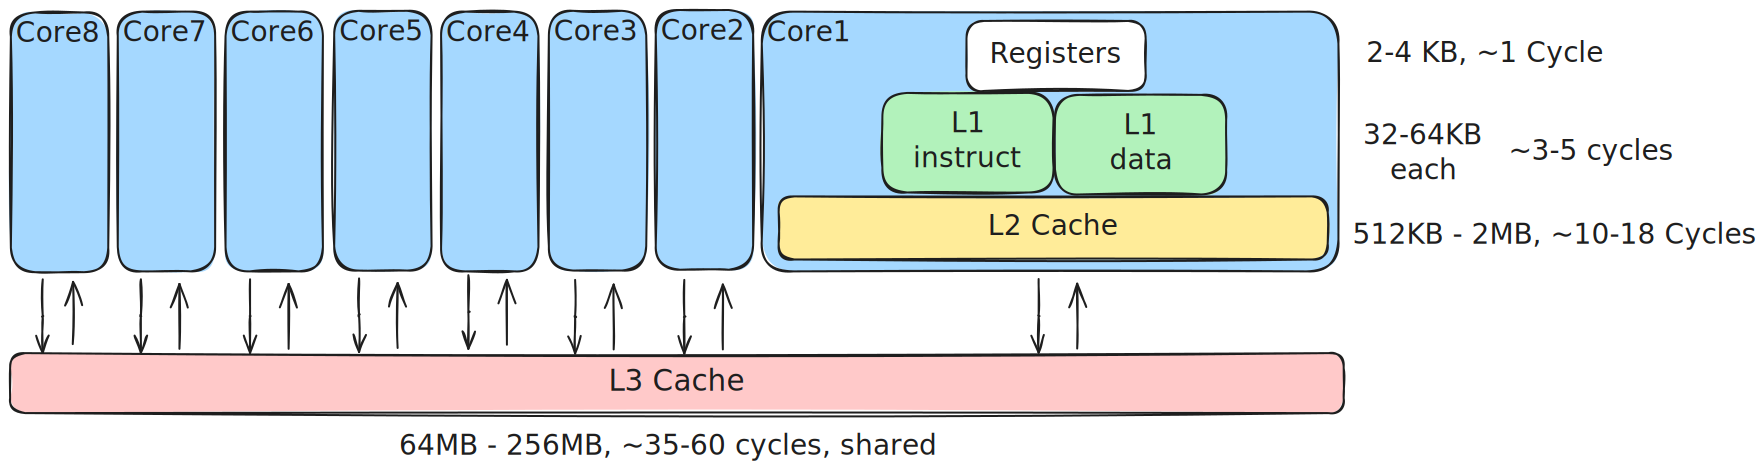
\includegraphics[width=0.95\linewidth]{cache_hierarchy.png}\\[0.3em]
    \caption{CPU cache hierarchy (registers, L1/L2/L3, main memory)}
    \label{fig:cache-hierarchy}
\end{figure}

\subsubsection{Cache Lines and Cache Locality}
A \texttt{Word} is the width of a standard register, on modern machines this is usually \texttt{8 Byte}. The architecture defines the size of a pointer, usually it's either \texttt{4 Byte} (on 32 bit architecture) or \texttt{8 Byte} (on 64 bit architecture). A \texttt{Cache Line} is the smallest contiguous chunk of memory that the CPU can load at once. Usually it's the size of \texttt{8 Word}. We will assume that 
\[
\texttt{CacheLine = 8 Word = 8 * 8 Byte = 64 Byte}.
\]

\subsubsection{Spatial vs Temporal Locality}
Spatial Locality means that if you access some element then you probably will access nearby elements as well, this is referred to as spatial locality. For example if you pull a variable into cache on a cache miss you pull in an entire cacheline, if you iterate through a large number of elements sequentially (potentially strided) the CPU will see this and pre-fetch memory to be used when it's needed (pipelining).
\begin{lstlisting}
for(auto i = 0zu; i < vec.size(); ++i) {
    // vec[i + 1] is already ready to be processed before this operation is done
    vec[i] += 1;
}
\end{lstlisting}

Temporal Locality means that if you access some element then you will probably access it again soon, so it makes sense to cache it.
\begin{lstlisting}
auto x = 1;
for(auto i = 0zu; i < vec.size(); ++i) {
    x += 2; // x remains in L1 cache, doesn't get evicted.
    vec[i] += x;
}
\end{lstlisting}

\subsubsection{False Sharing}
False sharing is a phenomenon that appears when you have two different threads write to elements on the same cache line. When thread a writes while thread b uses another value on the same cache line the cache line gets invalidated and so b has a cache miss and needs to pull the value into cache again despite it not having changed. To avoid this make sure that if two threads access memory often that they are not on the same cache line (easiest solution is to just pad to the next cache line, you can do that using the \texttt{std::hardware\_destructive\_interference\_size} constant.
\begin{lstlisting}
constexpr usize k_cacheline_size{std::hardware_destructive_interference_size};

struct Packed {
    int a{};
    int b{};
};

struct Seperated {
    alignas(k_cacheline_size) int a{};
    alignas(k_cacheline_size) int b{};
};

auto func_a(auto& Packed p) -> void {
    p.a = p.a + 1; // invalidates cache line that Packed lives on
}

auto func_b(auto& Packed p) -> void {
    p.b = p.b + 1; // invalidates cache line that Packed lives on
}

auto func_a_seperated(auto& Seperated p) -> void {
    p.a = p.a + 1; // Doesn't invalidate cacheline
}

auto func_b_seperated(auto& Seperated p) -> void {
    p.b = p.b + 1; // Doesn't invalidate cacheline
}

\end{lstlisting}

\subsection{Memory Layout and Alignment}
\subsubsection{Alignment vs Size}
\subsubsection{Tight Packing vs Padding}
\subsubsection{AoS vs SoA vs AoSoA}
Suppose you have the following representation of a physics owning entity represented as a fat struct
\begin{lstlisting}
struct Transform {
    Pos3 pos;
    Dir3 scale;
    Quaternion orientation;
};
struct Entity {
    u32 id{};
    Color3 color{};
    u32 visual_mask{};
    u32 hit_mask{};
    std::string name{};
    Transform transform{};
    std::unique_ptr<RigidBody> body{};
};
\end{lstlisting}
If we store our entities as
$$
std::vector<Entity> entities{};
$$
we have an (A)rray (o)f (S)tructs.

If we now want to update the position of all entites (for example by shifting them all, or syncing the transform with the underlying physics representation) then we'd have to load at least one \texttt{CacheLine} per entity which is a lot of wasted loading if we are only interested in the transform, for example
\begin{lstlisting}
sizeof(Transform) == sizeof(Pos3) + sizeof(Dir3) + sizeof(Quaternion) == 3 * 4 + 3 * 4 + 4 * 4 == 40
\end{lstlisting}
(assuming everything consists of 32 bit floats) while
\begin{lstlisting}
sizeof(Entity) == sizeof(u32) + sizeof(Color3) + sizeof(u32) + sizeof(u32)
                  + sizeof(std::string) + sizeof(Transform) + sizeof(std::unique_ptr)
               == 4 + 3 * 4 + 4 + 4 + 3 * 8 + 40 + 8
               == 96
\end{lstlisting}
Assuming things are aligned well we don't have to pull in 2 \texttt{CacheLine} but we still pull 24 Bytes of memory too much.

The code for shifting everything by \texttt{\{1.0f, 1.0f, 1.0f\}} is
\begin{lstlisting}
const Vec3 shift{1.0f, 1.0f, 1.0f};
for(auto& entity : entities) {
    entity.transform += shift;
}
\end{lstlisting}

We instead can store the individual components contiguously in memory
\begin{lstlisting}
TransformSOA {
    f32* pos_xs;
    f32* pos_ys;
    f32* pos_zs;
    f32* scale_xs;
    f32* scale_ys;
    f32* scale_zs;
    Quaternion* orientations;
}
\end{lstlisting}
and now we can load in three \texttt{CacheLine} to update 8 elements at a time, so we have 3 cache misses per 16 updates in the worst case. The pointers can for example store to a ArenaAllocator or some other contiguous storage like \texttt{std::vector} or \texttt{std::pmr::vector}). The update code becomes (assuming number of entities is divisible by 8 to avoid having to deal with boundary behavior)
\begin{lstlisting}
const auto shift_x = 1.0f;
const auto shift_x = 1.0f;
const auto shift_x = 1.0f;
for(auto i = 0zu; i < n_entities; ++i) {
    pos_xs[i] += shift_x;
    pos_ys[i] += shift_y;
    pos_zs[i] += shift_z;
}
\end{lstlisting}

A higher overhead but more SIMD aware storage method would be to use AoSoA, where we store arrays of blocks (here with element arrays of size 4 as I'm on NEON, can increase for AVX and AVX512):
\begin{lstlisting}
struct TransformBlock {
    std::array<f32, 8> pos_x;
    std::array<f32, 8> pos_y;
    std::array<f32, 8> pos_z;
    /*...*/
};
\end{lstlisting}

\subsubsection{SIMD Alignment Requirements}
\subsubsection{Practical Trade-offs (Bandwidth vs Compute)}

\subsection{CPU Microarchitecture}
\subsubsection{Pipelining}
\subsubsection{Branch Prediction and Speculative Execution}
\subsubsection{Out-of-Order Execution}

\subsection{GPU Architecture}
\subsubsection{Thread Blocks}
\subsubsection{Warps}
\subsubsection{Memory Coalescing}

\subsection{CPU--GPU Interaction}
\subsubsection{Asynchronous Execution}
\subsubsection{Synchronization Primitives}

\subsection{Benchmarking and Measurement}
\subsubsection{Sampling Benchmarks}
\subsubsection{Cache and Memory Profiling (perf, Valgrind)}

\newpage
\section{Concurrency}
\subsection{C++ Memory Model}
\subsubsection{Atomics}
There is only one atomic data type which is required to be lock free, namely \texttt{std::atomic\_flag}. Pretty much every core C++ data type has an atomic version, for example
\[
    \texttt{std::atomic<bool>}, \texttt{std::atomic<int>}, \texttt{std::atomic<float>}, \texttt{std::atomic<double>}
\]

It is important to check if those have hardware support (i.e. work lock free), this can be done by checking the compile time constant
\[
    \texttt{std::atomic<T>::is\_always\_lock\_free}
\]




\subsection{Multiple Threads}
\subsection{Multiple Processes}
\subsubsection{OpenMP}
\subsection{Data Structures}
\subsubsection{SPSC (Single Producer Single Consumer)}
\subsubsection{SPMC (Single Producer Multiple Consumer)}
\subsubsection{MPSC (Multiple Producer Single Consumer)}
\subsubsection{MPMC (Multiple Producer Multiple Consumer)}

\newpage
\section{Operating Systems}
\subsection{Process, Thread}
\subsection{Scheduling}
\subsection{CPU Virtualisation}
\subsection{Memory Virtualisation}
Suppose your pages are 16 bytes in size

\subsubsection{Paging, TLB}
Paging as opposed to segmentation slices up the availiable virtual memory into fixed-size pieces.

\newpage
\section{Networking}
\subsection{OSI Model}
\subsection{UDP}
\subsection{TCP/IP}

\newpage
\section{Trivia}
\subsection{Error \#323 on GCC}
There used to be a semi-famous issue where some compilers (notably GCC on x86) evaluated
floating-point expressions using 80-bit x87 registers, which could lead to results that were
“too correct” and therefore differ from other platforms and compilers
(see Reference~\ref{ref:floating-point-cpp}).

\newpage
\section{References}
\begin{itemize}
    \item \label{ref:floating-point-cpp}
    Egor Suvorov.\\
    \emph{Using Floating-point in C++: What Works, What Breaks, and Why}.\\
    CppCon 2025.  
    \url{https://www.youtube.com/watch?v=m83TjrB6wYw}

    \item \label{ref:cpp-software-design}
    Klaus Iglberger, \emph{C++ Software Design}.  
    O’Reilly Media, 2022.

    \item \label{ref:ostep}
    Remzi H. Arpaci-Dusseau, Andrea C. Arpaci-Dusseau,  
    \emph{Operating Systems: Three Easy Pieces}.  
    Arpaci-Dusseau Books.  
    \url{https://pages.cs.wisc.edu/~remzi/OSTEP/}
    
    \item \label{ref:pikus-efficient}
    Fedor Pikus, \emph{The Art of Writing Efficient Programs}.  
    Apress, 2021.

    \item \label{ref:cpp-concurrency}
    Anthony Williams, \emph{C++ Concurrency in Action} (2nd ed.).  
    Manning Publications, 2019.
\end{itemize}

\end{document}
